\section{Classification algorithms}

The objective of any \emph{classification algorithm} is to assign a class to each given data point so that some property is shared among all data points in a class. %TODO: in/of a class
For example, the main algorithm of this thesis evaluates the measured data of a $pp$-collision to estimate the type of the signal $B$ meson.
All classification algorithms used in this thesis are \emph{supervised machine learning algorithms}.
Such algorithms optimize the parameters $\theta$ of a given model $f$ so that the class predictions $\hat{y}=f(x|\theta)$ best fit to a given target $y$.
The process of optimizing these parameters is called \emph{training} and often involves minimizing a given \emph{loss function} $L(\hat{y}|y)$ that describes how the prediction $\hat{y}$ compares with the target $y$. 
The following sections describe the classification algorithms that are used in this thesis.

\subsection{Boosted Decision Trees}
\label{sec:BDT}

A \emph{Boosted Decision Tree} (BDT) is an ensemble of multiple different \emph{decision trees} trained and evaluated on the principles of \emph{gradient boosting}.
Decision trees are \emph{binary trees} with a decision condition at each node and a prediction score for each leaf.
The class prediction made on a given data point is based on a series of binary decisions on single features starting at the root and ending in a leaf of the decision tree.
The weighted sum of the prediction scores of all trees in a BDT is then transformed using the \emph{logistic function} to resemble an estimated probability that the given sample belongs to one of the classes.
In gradient boosting the decision trees are trained iteratively, so that at each step the weighted sum of all previous decision trees and the current decision tree minimizes a given loss function. 
The gradient of the loss function with respect to the model parameters is used to find this minimum.

\subsection{Neural Networks}
\label{sec:NN}

%\begin{figure}
%    \centering
%    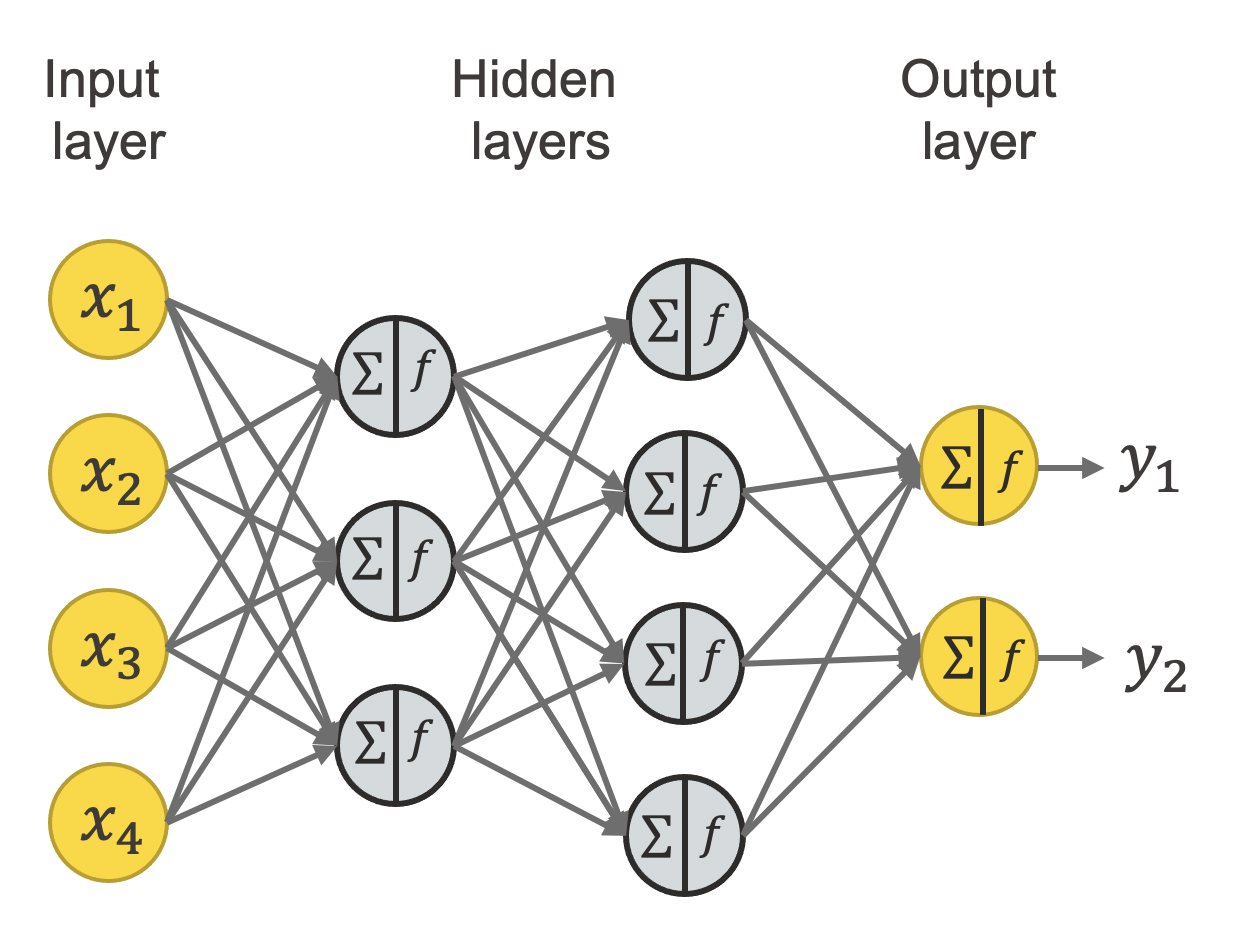
\includegraphics[width=0.5\textwidth]{images/NN_schematic.png}
%    \caption{Example of a fully connected, feedforward neural network \cite{NN_schematic}.}
%    \label{fig:NN_schematic}
%\end{figure}

A \emph{Neural Network} (NN) is a non-linear transformation of an input vector $\vec{x}$ into an output vector $\hat{\vec{y}}$.
This transformation is divided into multiple steps called layers.
The $n$th layer represents a vector $\vec{a}^{(n)}$, also called the \emph{activation}, that is calculated based on the values of the previous layer using the formula
\begin{equation*}
    \vec{a}^{(n)} = f^{(n)}\left( W^{(n)} \cdot \vec{a}^{(n-1)} + \vec{b}^{n} \right).
\end{equation*}
The \emph{weights}-matrix $W^{(n)}$ and the \emph{bias}-vector $\vec{b}^{(n)}$ are parameters of the model that have to be adjusted in the training process.
The \emph{activation function} $f$ can be any differentiable function that should be non-linear.
Used in this thesis are the activation functions
\begin{align*}
    f_\text{ReLU}(z) &= \max(0, z) \:\:\text{  and} \\
    f_\text{Sigmoid}(z) &= \frac{1}{1+e^{-z}} \, .
\end{align*}
The first layer of a NN is the input layer with the activation $a^{(0)}=\vec{x}$ and the last layer is the output layer with the activation used as $\hat{\vec{y}}$.
All other layers are called \emph{hidden layers}.

The iterative training of a NN uses a technique called \emph{backpropagation}.
As a first step, all weights of the NN are set to random values.
In each iteration of the training, the output of the NN is evaluated to estimate the gradient of the loss function with respect to all weights using the chain rule.
Based on this gradient, the weights are adjusted in the direction of the minimum of the loss function with a step size that is set by an \emph{optimizer}.
This thesis uses the loss function \enquote{binary cross entropy} in combination with the optimizer \enquote{Adam}\cite{adam}.

To reduce the \emph{overtraining} of the NN and increase its generalizability, this thesis uses regularization techniques called \emph{early stopping} and \emph{dropout}.
In early stopping, the performance of the model is evaluated on a validation dataset after each iteration, and the training is stopped when this performance does not increase over $N$ iterations.
This way, further adjusting of the NN to the training data is prevented, and only the best model with respect to the validation data is used.
In dropout, at each training iteration a smaller subset of the NN is trained by temporarily setting random rows in $W$ and $\vec{b}$ to 0.
The number of rows that are being disabled has to be set for each layer before training the NN.
Dropout leads to a more robust NN by reducing the co-dependence of pairs of activation elements.

\subsection{DeepSets}
\label{sec:DeepSet}

A \emph{DeepSet}\cite{deepset} is an extension of NNs to allow inputs of sets of vectors.
DeepSets can therefore be used to solve problems where the data of each sample contains a variable length list and where the solution should be invariant under permutations of this list.
In this thesis, a DeepSet is used to classify $pp$-collision events that contain different amounts of tracks of which the order in the data should not matter.

The underlying concept of a DeepSet is the function 
\begin{equation*}
    f(X) = \rho \left( \sum_{x \in X} \phi (x) \right)
\end{equation*}
which is invariant under permutations of the instances $x$ in a set $X$.
$\rho$ and $\phi$ represent NNs and can be vector-valued.
In principle, the sum could be replaced with any permutation invariant function, but in this thesis only sums are used.
In other words, a DeepSet contains a $\phi$-network and a $\rho$-network.
The $\phi$-network first extracts some features about each instance in the set.
The extracted feature values of all instances are then summed up and propagated into a $\rho$-network that calculates the final output.
Like NNs, DeepSets are also trained through backpropagation and the process is fully analogous to the training of a NN.




% A NN consists of multiple layers of (artificial) neurons to calculate an output vector $\hat{y}$ based on an input vector $x$.
% The amount of layers and the amount of neurons per layer can be arbitrarily chosen based on the complexity of the problem.
% A neuron represents a scalar number called activation that is calculated based on the weighted connections to the neurons of the previous % layer.
% The first layer of neurons is called the input layer and its activations are the values of $x$.


% A NN consists of multiple layers of (artificial) neurons to calculate an output vector $\hat{y}$ based on an input vector $x$.
% The amount of layers and the amount of neurons per layer can be arbitrarily chosen based on the complexity of the problem.
% A neuron calculates a scalar number called activation based on the activations of all neurons from the previous layer.
% The first layer of neurons is called the input layer and its activations are the values of $x$.
% When $a$ represents the activations of the previous layer, the linear activation of a single neuron in the next layer is
% \begin{equation*}
%     z = \sum_i w_i \cdot a_i + b \, .
% \end{equation*}
% $w_i$ is the weight associated with the connection to 
% 
% The activation of each other neuron is calculated through an activation function $f(z)$, where 
% \begin{equation*}
%     z = \sum_i w_i \cdot a_i + b \, .
% \end{equation*}
% $w_i$ is the weight of a connection between two neurons
% , the last layer is called the output layer and all layers in between are called hidden layers.
% 
% \cref{fig:NN_schematic} shows an example NN with 4 layers.
% Each neuron is represented as a circle and the arrows represent the weighted connections between two neurons.
% 
% 
% A NN passes an input vector $x$ through multiple layers of (artificial) neurons to calculate an output vector $\hat{y}$ that may have a % different length than $x$.
% The amount of layers and the amount of neurons per layer can be arbitrarily chosen based on the complexity of the problem.
% A schematic of a NN with 3 layers is shown in \cref{fig:NN_schematic}.
% Here, each neuron is represented by a circle and the arrows
% A neuron with an input vector $a$ first calculates a scalar 
% \begin{equation*}
%     z = \sum_i w_i \cdot a_i + b
% \end{equation*}
% called linear activation. 
% The vector $w$ and the scalar $b$ contain weights, that have to be optimized in the training process.
% Usually, this linear activation is then further transformed using an activation function.
% The activation functions used in this thesis are 
% \begin{align*}
%     \text{ReLU}(z) &= \max(0, z) & and \\
%     \text{Sigmoid}(z) &= \frac{1}{1+e^{-z}} \, .
% \end{align*}

